% 4yp.tex - 4th Year project report
% Max Jaderberg 2012

%-------------------------------
% Preamble
%-------------------------------
\documentclass[11pt, onecolumn, a4paper, final]{report} % 11pt font
\renewcommand{\familydefault}{\sfdefault} % sans-serif (Arial) font
\linespread{2} % double line spacing
\usepackage{amssymb,amsmath}
\usepackage[hang,small]{caption} % makes captions look nicer
\usepackage{graphicx}
\usepackage[margin=20mm]{geometry}
\usepackage{hyperref} % for hyperlinks

% for code listings
\usepackage{listings}
\usepackage{color}
\definecolor{dkgreen}{rgb}{0,0.6,0}
\definecolor{gray}{rgb}{0.5,0.5,0.5}
\definecolor{mauve}{rgb}{0.58,0,0.82}
\lstset{frame=tb,
  language=Java,
  aboveskip=3mm,
  belowskip=3mm,
  showstringspaces=false,
  columns=flexible,
  basicstyle={\small\ttfamily},
  numbers=none,
  numberstyle=\tiny\color{gray},
  keywordstyle=\color{blue},
  commentstyle=\color{dkgreen},
  stringstyle=\color{mauve},
  breaklines=true,
  breakatwhitespace=true
  tabsize=3
}

\title{The Intelligent Image}
\author{Max Jaderberg\\
	Keble College, University of Oxford}
\date{Trinity Term 2012}


%-------------------------------
% Document
%-------------------------------
\begin{document}

\maketitle

\begin{abstract}
In this report, I shall discuss some awesome stuff.
\end{abstract}

%-------------------------------
% Introduction
%-------------------------------
\chapter{Introduction}
The web contains billions of images, which are often the focus of attention on the web pages that include them. However, there is almost no information about the content of these images. Images on websites are purely binary data files, occasionally with some associated meta data included in the image's HTML\footnote{Hyper Text Markup Language \url{http://en.wikipedia.org/wiki/HTML}} code. Very little information is available about the image, let alone the objects or scenes contained within the image. The aim of this project is to create a system which automatically recognises the objects within these images, thus releasing the information within them. This is a large scale object retrieval problem.

There are a large number of applications which would benefit from having detailed information on the contents of images. With more knowledge on the objects contained within images, one can create more effective search engines, better cataloguing and classification systems, user interfaces which engage viewers more, and relevant advertising based on the content. Novel applications could also be built, for example, which retrospectively embed geographical information in the image binary by recognising where the image was photographed. The plethora of useful applications provides a great deal of motivation for this project.

\begin{figure}[ht]
\centering 
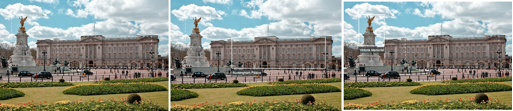
\includegraphics{images/intimage.png}
\caption{An example ``Intelligent Image'' showing the various hover over states}
\label{fig:intimage}
\end{figure}

The result of the project is that a query image is inputted, the objects contained within the image are recognised, and the image is returned with the recognised objects ``tagged'' i.e. the region of the object in the image is outlined and it can be clicked to give relevant information. In this way the standard image has been transformed into the ``intelligent image'' - one which knows about the contained scene and can offer up information to the consumer about it's contents.

Recognising a wide range of objects in an image is not a trivial problem. For such a system to be useful the following needed to be addressed:
\begin{itemize}
\item Acquire and filter enough data to create a model to perform matching on a large range of objects.
\item Create a retrieval system which provides accurate matching. False positive matching needs to be avoided as much as possible.
\item Ensure matching can be done quickly on a database of millions of objects.
\end{itemize}

To recognise millions of different objects, reference images are needed to create a model to match against. From the outset, Wikipedia\footnote{\url{http://en.wikipedia.org}} is used as the primary model data source. Wikipedia is a crowd-sourced online encyclopaedia with many images contained within the articles, and is considered an accurate source of information. In the system, each Wikipedia page defines an object, with the images in the article being used to provide the data to match against. The content of the Wikipedia article is used to give the user further information about the object. A web crawler was written to extract the relevant images of desired Wikipedia pages and create the image database. Filtering is also performed to ensure only useful images are included in the database. The data sources are fully explained in Chapter~\ref{chpt:data}.

Object retrieval uses a method employing a bag-of-words model. This builds upon the work described in x and y, more information of which is provided in Chapter~\ref{chpt:background}. The visual words in the image database from Wikipedia are precomputed. At run time, the words in the query image are computed and searched against the database of precomputed words to find the top image matches. The top matches are spatially verified, with the first verified image being the result. Subsequent improvements to the base line system (described fully in Chapter~\ref{chpt:system}) were made, including geometric improvements to the spatial verification and descriptors used to increase speed and accuracy of spatial verification, and matching improvements through query expansion using crowd-sourced data (dubbed ``Turbo-boosting'') from Microsoft's Bing\footnote{\url{http://www.bing.com}} search engine. The geometric improvements and turbo-boosting is reported in Chapter~\ref{chpt:geoimprovements} and Chapter~\ref{chpt:turboboosting} respectively.

Finally a website was developed to provide a front end interface for the system. A user can simply navigate to the website and upload an image. They then start the automatic tagging process, during which a realtime log of the process is displayed. After the query is complete, the intelligent image is displayed, which the user can interact with, see the names of the objects contained within the image, and click on the object to go to it's Wikipedia page. The software architecture of the website and the backend systems is explored in Chapter~\ref{chpt:architecture}. The result is a realtime automatic tagging system which could recognise, for example, all the buildings in a tourist's photo album of London in seconds.

The aim of the project is to work towards recognising every object on Wikipedia, however due to time restraints a subset of objects was used for development and testing of the project. The subset chosen were the pages that appear on the Wikipedia page ``List of Structures in London''\footnote{\url{http://en.wikipedia.org/wiki/List_of_structures_in_London}}.
	

%-------------------------------
% Background
%-------------------------------
\chapter{Background}
\label{chpt:background}


%-------------------------------
% Data
%-------------------------------
\chapter{Data}
\label{chpt:data}
There are three main datasets used by the application: the images from Wikipedia used to build the database of objects (Section~\ref{sec:modelimages}), the images from Microsoft Bing used for the Turbo-boosting (Section~\ref{sec:turboimages}) and the images from Google Images used for validation and testing (Section~\ref{sec:validationimages}). This chapter describes the various datasets and how they are acquired.

\section{Model Images}
\label{sec:modelimages}
The model comprises of a dataset of images which depict the objects that are to be able to be recognised. To enable an object to be recognised, the object must be represented by one or more images contained within the model. For example, the object ``Tower Bridge'' will be best represented by multiple images of Tower Bridge taken at different angles and focussing on different features. Wikipedia was used as the source of the images to represent the objects described by the Wikipedia pages. The resulting representations work well - an example object representation is shown in Figure~\ref{fig:towerbridge}.

\begin{figure}[htb]
\centering 
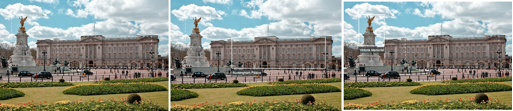
\includegraphics{images/intimage.png}
\caption{The representation of the object ``Tower Bridge'' by images}
\label{fig:towerbridge}
\end{figure}

Each page of Wikipedia that contains images represents an object which can be matched. The database of images which is used to build the model is simply created by visiting each page on Wikipedia for the objects desired and downloading the relevant images contained on the web page, labelling that image as being associated with the object. A script automates this process of building the model database.

\begin{figure}[htb]
\centering 
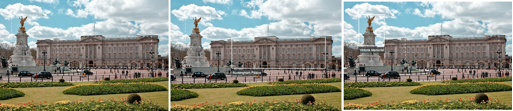
\includegraphics{images/intimage.png}
\caption{The Wikipedia page for ``Tower Bridge''. Note the images contained are those used in the model to represent this object.}
\label{fig:wikipage}
\end{figure}

To automate the downloading of object images from Wikipedia, Python\footnote{\url{http://www.python.org}} is used. WIkipedia offers a public application programming interface (API) over HTTP as it is built on the MediaWiki framework\footnote{The MediaWiki framework was originally developed for Wikipedia and provides an API over HTTP as standard. \url{http://www.mediawiki.org/wiki/API} provides documentation for the API.}, however it is cumbersome and not easy to consume. Instead, a web crawler was written to explore Wikipedia pages and extract the relevant images. 

A crawler object in Python finds all the images and notes the urls of them for subsequent download. Firstly, the HTML of the Wikipedia page must be downloaded, as it appears to a web browser (an example of a web browser being Google Chrome). However, Wikipedia does not allow crawlers and automated bots to access its web pages. To overcome this, the HTTP header\footnote{\url{http://www.w3.org/Protocols/rfc2616/rfc2616.html} describes the Hyper Text Transport Protocol and the various header fields.} of the crawler is edited to emulate that of a browser. This is implemented using the urllib2 library\footnote{\url{http://docs.python.org/library/urllib2.html}}. The code shown in Listing~\ref{lst:crawler} shows an example of how to read the HTML of the main Wikipedia homepage. The HTML document for each Wikipedia page is parsed using the BeautifulSoup library\footnote{\url{http://www.crummy.com/software/BeautifulSoup/}}. All the anchor elements are found and stored for further crawling. The images contained within the HTML are also found by looking within the part of the HTML document that is unique to the specific Wikipedia page (see Listing~\ref{lst:beautifulsoup}).

\lstset{language=Python,caption=The code used to gain access to Wikipedia's content using a crawler by emulating a browser.,label=lst:crawler}
\begin{lstlisting}
### Python
import urllib2
# Emulate the user agent as that of a browser
user_agent = "Mozilla/5.0 (Macintosh; U; Intel Mac OS X; en-US; rv:1.8.1.7) Gecko/2007091417 Firefox/2.0.0.7"
headers = {"User-Agent": user_agent}
# Request the webpage
req = urllib2.Request("http://en.wikipedia.org", headers=headers)
resp=urllib2.urlopen(req)
# Read the HTML of the response
html = resp.read()
\end{lstlisting}


\lstset{language=Python,caption=Parsing the Wikipedia article HTML document to find the relevent images.,label=lst:beautifulsoup}
\begin{lstlisting}
### Python
def _get_content_body(self, soup):
        main_content = soup.find('div', {"class": "mw-content-ltr"})
        if main_content is None:
            return None
        # remove navboxes
        navboxes = main_content.findAll('table', {'class': 'navbox'})
        [navbox.extract() for navbox in navboxes]
        return main_content

def _get_image_links(self, soup):
	return soup.findAll('a', {'class': 'image'})
	
# Parse the HTML
soup = BeautifulSoup(html)
# Get the main article body
soup = _get_content_body(soup)
# Get a list of image links
image_links = _get_image_links(soup)
\end{lstlisting}



\section{Turbo-boosting Images}
\label{sec:turboimages}

\section{Validation Images}
\label{sec:validationimages}


%-------------------------------
% Base line system
%-------------------------------
\chapter{Base line system}
\label{chpt:system}

%-------------------------------
% Software architecture
%-------------------------------
\chapter{Software architecture}
\label{chpt:architecture}


%-------------------------------
% Geometric Improvements
%-------------------------------
\chapter{Geometric Improvements}
\label{chpt:geoimprovements}


%-------------------------------
% Turbo-boosting
%-------------------------------
\chapter{Turbo-boosting}
\label{chpt:turboboosting}


%-------------------------------
% Summary
%-------------------------------
\chapter{Summary}


%-------------------------------
% References
%-------------------------------
\begin{thebibliography}{99}

	\bibitem{turcot09}
		P. Turcot and D. G. Lowe.
		Better matching with fewer features: The selection of useful features in large database recognition problems
		In \emph{WS-LAVD, ICCV}, 2009.
	  
\end{thebibliography}

\end{document}